% A skeleton file for producing Computer Engineering reports
% https://kgcoe-git.rit.edu/jgm6496/KGCOEReport_template

\documentclass[CMPE]{../KGCOEReport}

% The following should be changed to represent your personal information
\newcommand{\classCode}{CMPE 460}  % 4 char code with number
\newcommand{\name}{Andrei Tumbar}
\newcommand{\LabSectionNum}{2}
\newcommand{\LabInstructor}{Beato}
\newcommand{\TAs}{Xavier Brooks\\
Diana Yakobchuk}
\newcommand{\exerciseNumber}{2}
\newcommand{\exerciseDescription}{UART Driver}
\newcommand{\dateDone}{1/21/2022}

\usepackage{tikz}
\usepackage{circuitikz}
\usetikzlibrary{calc}
\usepackage{multirow}
\usepackage{titlesec}
\usepackage{float}
\usepackage{lmodern}
\usepackage{pgfplots}
\usepackage{siunitx}
\usepackage{subcaption}
\usepackage{graphicx}
\usepackage[usestackEOL]{stackengine}
\usepackage{scalerel}
\usepackage[T1]{fontenc}
\usepackage{amsmath}
\usepackage{pdfpages}


\def\code#1{\texttt{#1}}

\begin{document}
    \maketitle
    \section*{Description}

    The focus of this laboratory exercise was to implement a basic UART driver for
    MSP432 devices. The driver was driven via polling the status of the peripheral device
    in order to send and receive data.

    \section*{Part 2}

    After the ports and pins of the UART peripheral device were found, the next step was
    to initialize the device to work over a serial interface. A baud rate of 9600 was chosen
    to communicate with meaning a proper prescaler would need to be chosen to divide the
    input clock to the desired frequency of the peripheral.

    With the \code{EUSCI\_A0} device initialized, the transmission side was tested by
    transmitting a simple string across the UART.

    \begin{figure}[h!]
      \centering
      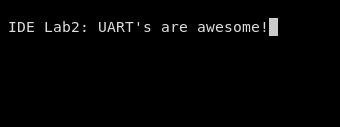
\includegraphics[width=8cm]{part2}
      \caption{Screenshot of basic UART transmission on MSP432}
      \label{fig:part2}
    \end{figure}

    Figure \ref{fig:part2} shows the correct operation of the UART transmitter
    by properly printing the given string to the screen. Note that the newline characters
    work as intended by placing a newline before the sentence.

    \section*{Part 3}

	Knowing that the transmission side of the UART is operational, the next step
	is to test the receiver. To do this, an echo program was made to take user input
	and print out the received bytes.

    \begin{figure}[h!]
      \centering
      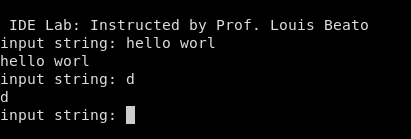
\includegraphics[width=8cm]{part3}
      \caption{Screenshot of echo program user interface}
      \label{fig:part3}
    \end{figure}

	Because the maximum number of characters is capped to 10 bytes as to not overfill our
	input buffer, attempting to input \code{hello world} will cause the input to break
	early and print the first 10 characters. Notice the second input string in Figure
	\ref{fig:part3} is only a single character, this is also handled properly. 

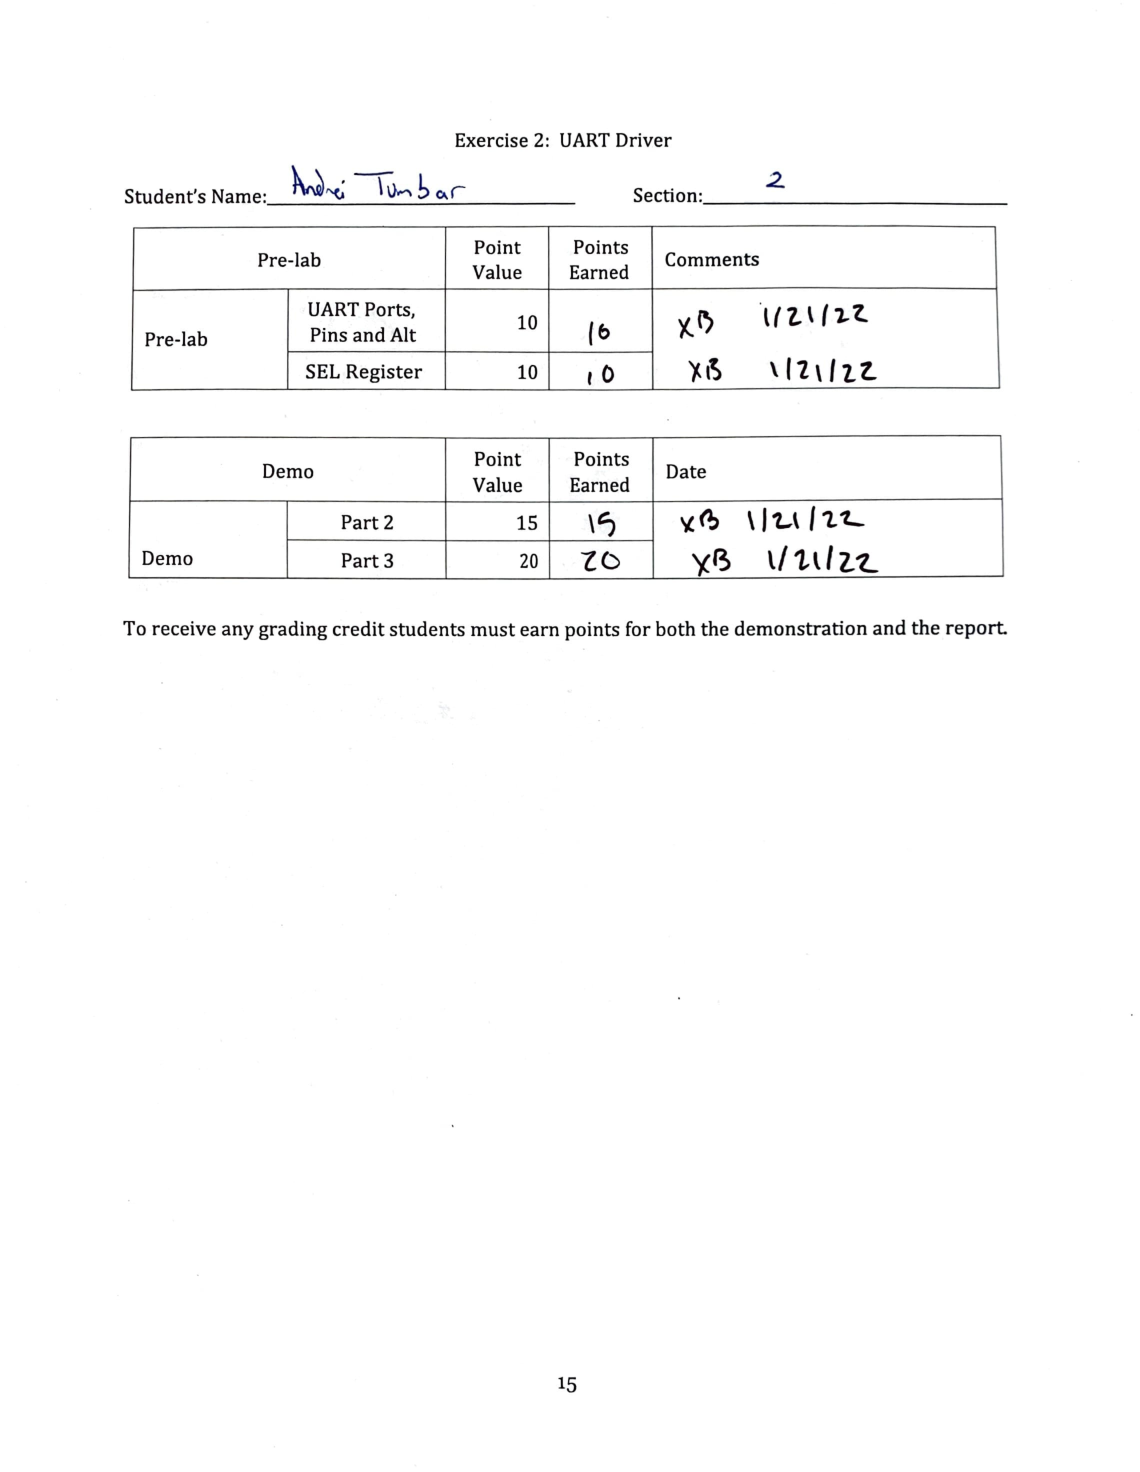
\includepdf[pages=-,pagecommand={},width=\textwidth]{signoff2.pdf}

\end{document}
